\section{Introdução}

Por volta de 20.000 aC. o homem já utilizava uma espécie de dispositivo que viabilizava a troca de calor, conhecido como panela de cozinhar. Arquimedes de Siracusa, por volta de 212 A.C., criou o primeiro dispositivo de calor destinado ao uso comercial e público, o canhão a vapor. Heron, em 120 A.C., criou outro dispositivo, a esfera gigante. Entretanto, somente em 1763 o trocador de calor foi lançado, com a criação da máquina a vapor de James Watt; \cite{abdallah_2018_multi}

Atualmente, os trocadores de calor apresentam grande importância por fornecer Alta eficiência térmica no processo de transferência de calor, baixo custo de instalação, alta performance, com baixo volume retido, fácil desmontagem para manutenção e, por ser um equipamento geralmente desmontável, permite o ajuste da capacidade do trocador adicionando ou removendo placas do equipamento.\cite{abdallah_2018_multi}

Por definição, os trocadores de calor são equipamentos responsáveis por realizar troca térmica entre dois ou mais fluidos a diferentes temperaturas, podendo ou não ocorrer mudança de fase dos fluidos. Adota-se trocador de calor ao equipamento que não promove a mudança de fase dos fluidos, enquanto os que ocorrem essa alteração recebem nomes específicos, como evaporadores, condensadores, refervedores ou vaporizadores. Dentre os variados campos de aplicação desses equipamentos estão indústrias de processo, química e alimentícia, resfriamento e/ou aquecimento de ambientes, condicionamento de ar, recuperação de calor, produção de energia, radiadores de automóveis e veículos espaciais.\cite{abdallah_2018_multi}
Os trocadores de calor possuem configurações dos mais variados tipos para as mais variadas aplicações. O trocador de calor que será dimensionado e selecionado neste trabalho será o do tipo casco e tubo, cuja configuração geral segue exemplificada na figura \ref{fig:fig1}: \cite{abdallah_2018_multi, incase_2022_trocador}
\\
\begin{figure}[h]
	\centering
	\caption{Trocador de calor de casco e tubo}
	\label{fig:fig1}
	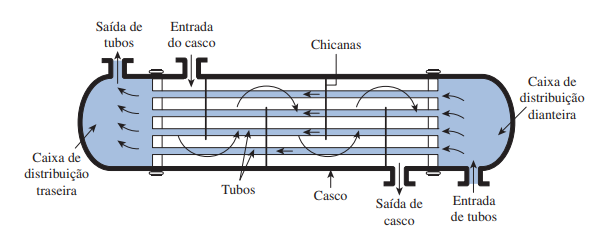
\includegraphics[width=1\linewidth]{imagens/fig1}
	
	\text{Fonte: \cite{incase_2022_trocador}}
\end{figure}

\subsection{Tipos principais de trocadores de calor e configuração de escoamentos}
Os dois principais tipos de trocadores de calor encontrados nas aplicações rotineiras são os seguintes:
\begin{itemize}
	\item Casco e Tubo;
	\item Tubo duplo;
	\item Placas Paralelas;
\end{itemize}

O trocador de casco e tubos é o mais utilizado na indústria de refino de petróleo, uma vez que possui amplas faixas de vazão, temperatura e pressão \cite{orgeda_2020_trocadores}. Em geral, é o único que pode ser aplicado em processos que necessitam de grandes áreas de troca de calor, acima de \(5000m^2\), pressões acima de \(30bar\) e temperaturas superiores a \(260^oC\) \cite{orgeda_2020_trocadores}. Aliado a isso, pode operar com líquidos, gases ou vapores, como condensador ou vaporizador, em posição horizontal ou vertical, de acordo com as necessidades operacionais a serem determinadas \cite{orgeda_2020_trocadores}. 

\begin{figure}[h]
	\centering
	\caption{Trocador de calor com múltiplos tubos internos}
	\label{fig:fig2}
	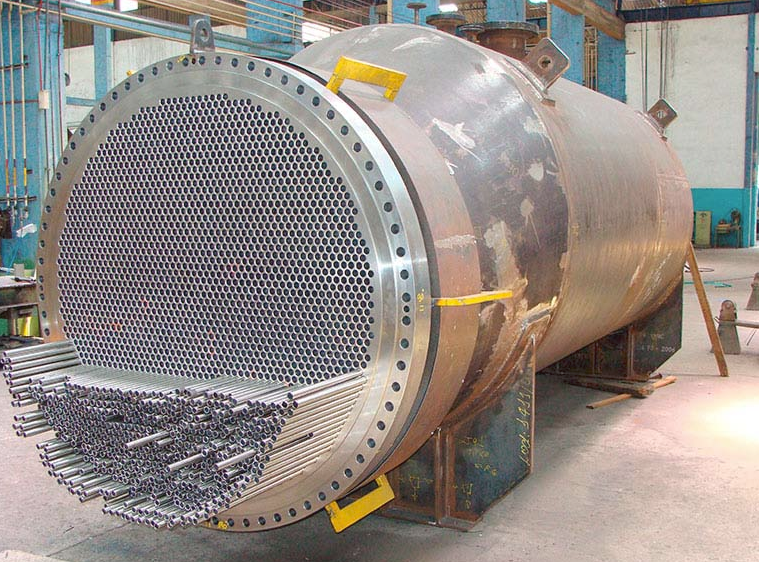
\includegraphics[width=.7\linewidth]{imagens/fig2}
	
	\text{Fonte: \cite{incase_2022_trocador}}
\end{figure}
O modelo mais simples de trocador de calor é o chamado trocador de tubo duplo, que consiste essencialmente em dois tubos concêntricos, em que um dos fluidos escoa pelo tubo de diâmetro menor e o outro escoa pelo espaço anular entre os dois tubos. Geralmente, este tipo de trocador apresenta dois trechos retos com conexões nas extremidades dos tubos.

\begin{figure}[h]
	\centering
	\caption{Esquemático: Trocador de tubo duplo}
	\label{fig:fig3}
	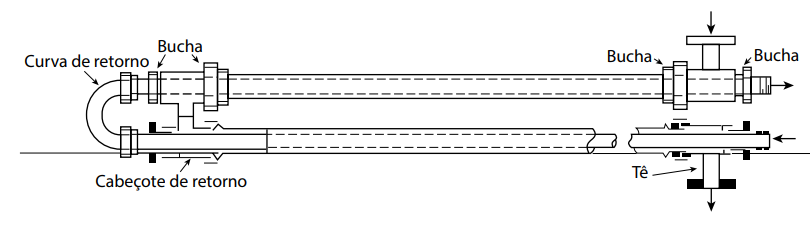
\includegraphics[width=.8\linewidth]{imagens/fig3}
	
	\text{Fonte: \cite{orgeda_2020_trocadores}}
\end{figure}

O fluxo do escoamento dos fluidos que exercerão a troca térmica ao longo dos componentes do trocador de calor em questão define papel crucial no desempenho do trocador de calor. Em suma, os perfis de temperatura de ambos os fluidos que trocam calor apresentam perfis diferentes em função da direção dos escoamentos. Em geral, são utilizados dois tipos de escoamentos em trocadores de calor: escoamento paralelo e contracorrente.

 Para o escoamento paralelo, as temperaturas dos dois fluidos tendem a se aproximar e a diferença de temperatura ao longo do trocador diminui significativamente. De outra forma, para o escoamento contracorrente, o fluido frio pode sair do equipamento mais quente do que o próprio fluido quente sai, e as diferenças de temperatura entre os dois fluidos ao longo do trocador apresentam menor variação \cite{cengel_2012_transferencia}. A figura \ref{fig:fig4} representa de forma simplificada estas duas situações:
 
 
 \begin{figure}[h]
 	\centering
 	\caption{Arranjos de escoamento em trocadores de calor e seus perfis de temperatura associados.}
 	\label{fig:fig4}
 	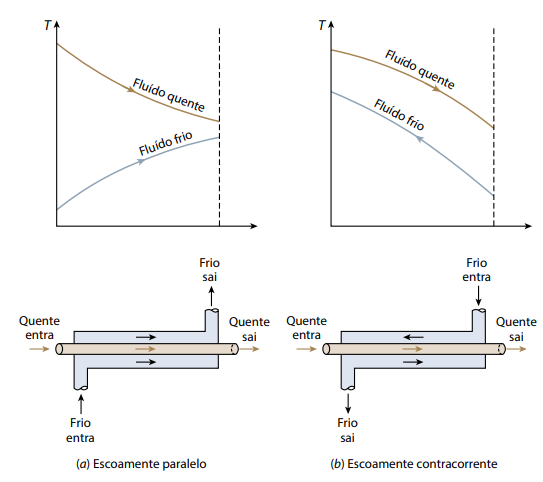
\includegraphics[width=.7\linewidth]{imagens/fig4}
 	
 	\text{Fonte: \cite{cengel_2012_transferencia}}
 \end{figure}
 
 